\chapter{Objetivos, hipótesis y factores}
\label{cap:objetivos}

Datos de entrada, lo que se promete y lo que se hipotetiza. La figura del cierre ata OE1--OE4 al
Capítulo~\ref{cap:metodologia}.

\section{Línea de base / datos iniciales}

No hay mediciones previas del grupo. La línea de base son los archivos con los que trabajaría el
modelo:

\begin{itemize}
  \item \textbf{Entrada principal:} contratos OpenAPI~3.x del sector bancario (objeto de estudio,
        Cap.~1 §1.4).
  \item \textbf{Referencia de contraste:} especificaciones de \ServiceDomain{} BIAN (\Behavior{},
        \BusinessObject{}, relaciones de control).
  \item \textbf{Producto esperado:} representaciones normalizadas, scores S/E/C y
        \AlignmentScore{} con clasificación por niveles.
\end{itemize}

Quedan fuera de esta línea de base las implementaciones en producción, el tráfico \textit{runtime} y
los artefactos de testing automatizado (delimitación §1.6). Los ejemplos del Cap.~1 (Tabla~1.4,
Anexo~F) ilustran el procedimiento pero \textbf{no fijan un caso piloto único}: el diseño aplica a
cualquier par contrato OpenAPI bancario --- \ServiceDomain{} BIAN que cumpla los criterios de
inclusión definidos en el plan.

\section{Objetivo superior}

El \textbf{objetivo superior} es lo que pasaría en un banco \textit{si} el modelo existiera y se
usara. No es el objetivo técnico de Guía~1. Sirve para no perder de vista por qué importa:

\begin{quote}
  Contar con un procedimiento verificable que permita a equipos de arquitectura y gobernanza de APIs
  \textbf{cuantificar la coherencia} entre contratos OpenAPI y modelos BIAN \textbf{antes} del
  despliegue o la certificación, reduciendo retrabajo en adaptadores, ensayo--error en integraciones
  y deriva entre la capa técnica y el modelo de negocio de referencia.
\end{quote}

Guía~1 no pone eso en producción (§1.6). Entrega el modelo y el procedimiento. El software y el
piloto a escala son otra entrega.

\section{Objetivo general (técnico)}

\textbf{Diseñar} cómo se calculan S, E, C y el \AlignmentScore{} de un contrato OpenAPI frente a
un \ServiceDomain{} BIAN, y dejarlo escrito de modo que otro pueda seguir los mismos pasos
(Anexo~C).

La unidad de medición es el par \texttt{contrato $\times$ Service Domain}. Sale un
\AlignmentScore{} en $[0,1]$ y un nivel. Esa es la variable dependiente. S, E, C y la
completitud de OE1 son insumos, no el resultado que cierra la tesis.

OE1 prepara los artefactos. OE2 responde P1 (E). OE3 responde P2 (S). OE4 junta C, el score y
las tipologías (P3--P4). Tabla~\ref{tab:objetivos-especificos}, \Cref{fig:cadena-objetivos} y
Anexo~C.

\section{Objetivos específicos}

OE1--OE4 son transformaciones, no deseos. Encajan en las cinco fases del modelo
(§\ref{sec:objetivos-metodologia}).

\begin{table}[H]
  \centering
  \caption{Objetivos específicos como transformaciones}
  \label{tab:objetivos-especificos}
  \small
  \begin{tabular}{@{}p{0.08\textwidth}p{0.22\textwidth}p{0.30\textwidth}p{0.30\textwidth}@{}}
    \toprule
    \textbf{ID} & \textbf{Subproblema} & \textbf{Entrada} & \textbf{Salida (producto)} \\
    \midrule
    \textbf{OE1} &
    Adquisición y normalización &
    Contrato OpenAPI bancario + \ServiceDomain{} BIAN &
    Representaciones normalizadas comparables (\textit{paths}, \textit{schemas},
    \Behavior{}, \BusinessObject{}) \\
    \textbf{OE2} &
    Alineación estructural (P1) &
    Representaciones normalizadas &
    Matriz de correspondencias + \StructuralScore{} (E) $\in [0, 1]$ \\
    \textbf{OE3} &
    Alineación semántica (P2) &
    Representaciones normalizadas &
    Matriz de similitud + \SemanticScore{} (S) $\in [0, 1]$ \\
    \textbf{OE4} &
    Evaluación integrada (P3--P4) &
    \StructuralScore{} (E), \SemanticScore{} (S) y representaciones normalizadas (OE1) &
    \CoverageScore{} (C); \AlignmentScore{}; clasificación (Alta/Media/Baja/Nula); tipologías \\
    \bottomrule
  \end{tabular}
\end{table}

La \textbf{Fase~1} del modelo (diseño del procedimiento y definición de scores) corresponde al
marco metodológico general del plan y no se confunde con OE1--OE4, que son
transformadores sucesivos sobre los artefactos.

\section{Hipótesis}

Una por OE. El factor y el ratio de cada una están en la Tabla~\ref{tab:variables}; aquí va el
contenido.

\begin{enumerate}
  \item \textbf{H1 (OE1).} Si OpenAPI y BIAN se normalizan al mismo modelo intermedio, S, E y C se
        pueden calcular sobre esas tablas (completitud de la extracción como ratio).
  \item \textbf{H2 (OE2).} Jaccard de nombres, path y verbo HTTP ---la caja de
        \textit{schema matching} de Shvaiko y Euzenat (2005)--- alcanza para un E que distinga
        un par razonable de uno forzado.
  \item \textbf{H3 (OE3).} Similitud de texto (El Bayadh et al., 2015; Chandrasekaran y Mago,
        2022), y más adelante embeddings, separan un concepto alineado de un falso amigo de
        modelado. Eso es S.
  \item \textbf{H4 (OE4).} Con $\alpha=\beta=\gamma=1/3$ el \AlignmentScore{} se puede leer como
        Alta/Media/Baja/Nula. Cambiar los pesos (sensibilidad) no debe invertir el relato de una
        instancia, solo el número.
\end{enumerate}

La Fase~1, la del diseño, asume que partir en S, E y C es mejor que un único ``índice de
coherencia'' opaco. El Anexo~C lo deja en filas.

\section{Factores y ratios de la investigación}

Los \textbf{factores} son las condiciones de diseño cuya variación puede contrastarse en una
validación empírica posterior; los \textbf{ratios} son los resultados numéricos medidos (scores y
clasificación). Los \textbf{parámetros de control} mantienen constantes otras condiciones para
comparar el efecto de cada factor.

\begin{table}[H]
  \centering
  \caption{Factores y ratios por objetivo específico}
  \label{tab:variables}
  \small
  \begin{tabular}{@{}p{0.08\textwidth}p{0.22\textwidth}p{0.22\textwidth}p{0.36\textwidth}@{}}
    \toprule
    \textbf{OE} & \textbf{Factores} & \textbf{Ratios (resultados)} & \textbf{Parámetros de control} \\
    \midrule
    \textbf{Artefacto (OG)} &
    Modelo S/E/C; pesos $\alpha$, $\beta$, $\gamma$ &
    \textbf{\AlignmentScore{} + clasificación} (VD global del artefacto) &
    Instancia \texttt{contrato $\times$ SD}; $\alpha+\beta+\gamma=1$; umbrales §1.4 \\
    \midrule
    \textbf{OE1} &
    Esquema de representación intermedia &
    Completitud de extracción (elementos extraídos / esperados) &
    Versión fija del contrato OpenAPI y del \ServiceDomain{} BIAN; herramientas de \textit{parsing} fijas \\
    \textbf{OE2} &
    Estrategia de \textit{schema matching} &
    \StructuralScore{} $\in [0, 1]$ &
    Mismo conjunto normalizado de OE1; umbral de correspondencia fijo \\
    \textbf{OE3} &
    Técnica de similitud semántica (embeddings, ontología, híbrido) &
    \SemanticScore{} $\in [0, 1]$ &
    Mismo corpus de términos; umbral de similitud fijo \\
    \textbf{OE4} &
    Pesos de agregación ($\alpha$, $\beta$, $\gamma$) &
    \CoverageScore{} (ratio parcial); contribuye a \AlignmentScore{} &
    $\alpha + \beta + \gamma = 1$ fijos; mismos S, E, C; taxonomía Tabla~\ref{tab:tipologias} \\
    \bottomrule
  \end{tabular}
\end{table}


Los indicadores y métricas detallados por fase se documentan en la matriz de consistencia (Anexo~C).

\section{Figura de cadena de objetivos}

La \Cref{fig:cadena-objetivos} cierra este capítulo: secuencia de transformaciones desde los
artefactos de entrada hasta el \AlignmentScore{} integrado.

\begin{figure}[H]
  \centering
  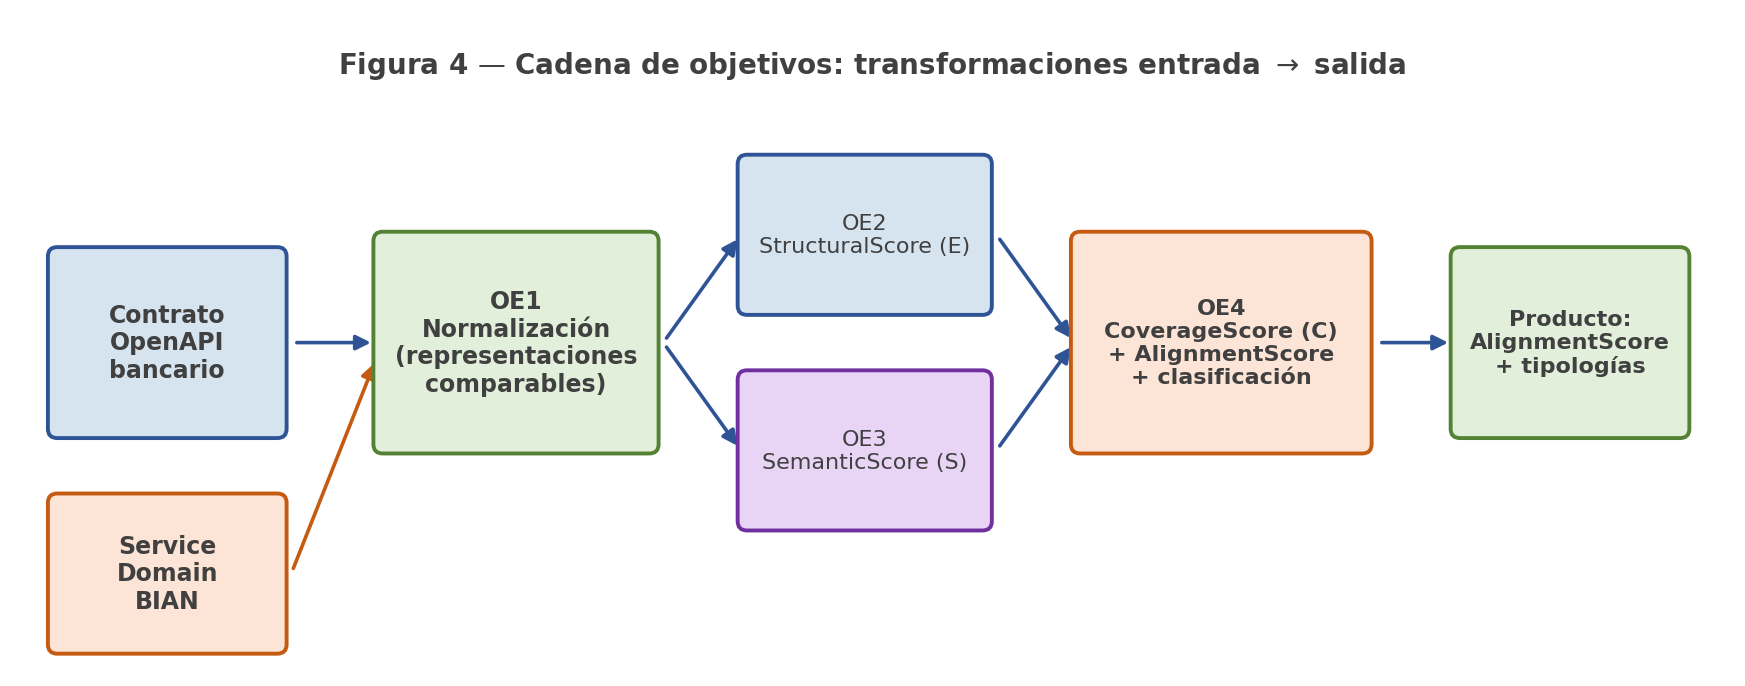
\includegraphics[width=0.98\textwidth]{Figura_04_Cadena_Objetivos}
  \caption{Cadena de objetivos: normalización $\rightarrow$ scores parciales $\rightarrow$ score global.
           Fase~1 (diseño del modelo) precede a OE1; ver Anexo~C.}
  \label{fig:cadena-objetivos}
\end{figure}
